\subsection*{i. El estado que ha realizado la menor cantidad de órdenes. Se debe mostrar también el total de ordenes que haya entregado.}
\addcontentsline{toc}{subsection}{i.}

Primero, se realiza un JOIN entre \texttt{customer} y \texttt{orders} con el ID de cliente de ambas tablas. Luego, los registros se agrupan por el estado de vivienda de los clientes, y se realiza un conteo por id (que, como es único y no nulo, es en escencia un conteo de filas), lo que realiza un conteo de registros por estado y, finalmente, el resultado se ordena de forma descendente.

La notación en álgebra lineal no permite formular nativamente la operación \texttt{LIMIT}, pero se puede observar, según el primer registro de la columna, que el estado con más pedidos es California, con un registro total de 1200.

Expresión:
\begin{itemize}[nosep]
\item [\ ] $\tau_{totalorders\ desc}$
\item [\ ] $($
        \begin{itemize}
            \item [\ ] $\gamma_{customer.state;\ count(orders.orderid)\rightarrow totalorders}$
            $($
            \begin{itemize}
                \item [\ ] $customer$
                    \begin{itemize}
                        \item [\ ] $\bowtie_{customer.customerid=orders.customerid}$
                    \end{itemize}
                \item [\ ] $orders$
            \end{itemize}
            $)$
        \end{itemize}
    $)$
\end{itemize}


Resultados obtenidos:

\begin{figure}[h!]
\centering
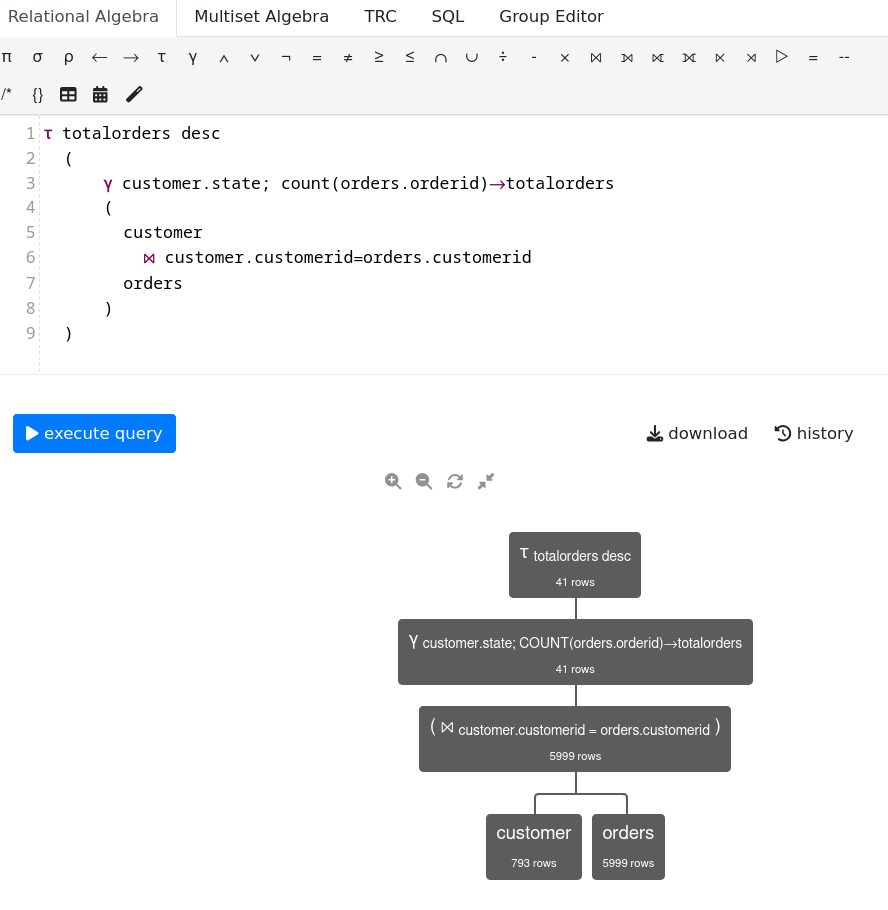
\includegraphics[width=0.8\textwidth]{imagenes/result2I1.png}
\caption{Consulta y árbol generado.}
\end{figure}

\begin{figure}[h!]
\centering
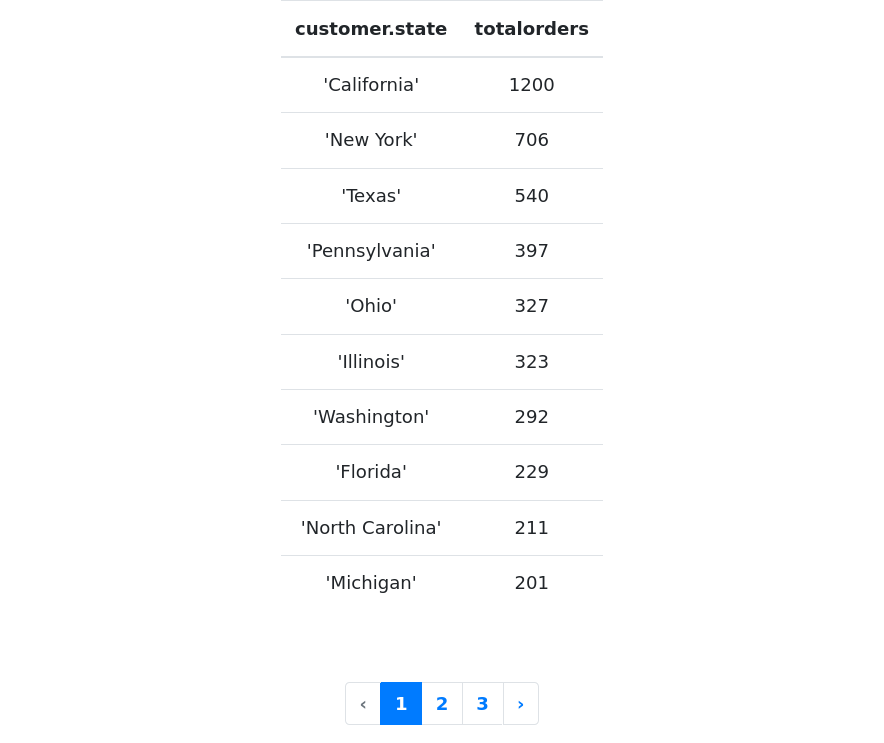
\includegraphics[width=0.8\textwidth]{imagenes/result2I2.png}
\caption{Resultado de consulta.}
\end{figure}